%%%%%%%%%%%%%%%%%%%%%%%%%%%%%%%%%%%%%%%%%
% Structured General Purpose Assignment
% LaTeX Template
%
% This template has been downloaded from:
% http://www.latextemplates.com
%
% Original author:
% Ted Pavlic (http://www.tedpavlic.com)
%
% Note:
% The \lipsum[#] commands throughout this template generate dummy text
% to fill the template out. These commands should all be removed when 
% writing assignment content.
%
%%%%%%%%%%%%%%%%%%%%%%%%%%%%%%%%%%%%%%%%%

%----------------------------------------------------------------------------------------
%	PACKAGES AND OTHER DOCUMENT CONFIGURATIONS
%----------------------------------------------------------------------------------------

\documentclass{article}

\usepackage{listings}
\usepackage{mathtools}
\usepackage{fancyhdr} % Required for custom headers
\usepackage{lastpage} % Required to determine the last page for the footer
\usepackage{extramarks} % Required for headers and footers
\usepackage{graphicx} % Required to insert images
\usepackage{lipsum} % Used for inserting dummy 'Lorem ipsum' text into the template
\usepackage{caption}
\usepackage{subcaption}
\usepackage{amsmath}
\usepackage{url}

% Margins
\topmargin=-0.45in
\evensidemargin=0in
\oddsidemargin=0in
\textwidth=6.5in
\textheight=9.0in
\headsep=0.25in 

\linespread{1.1} % Line spacing

% Set up the header and footer
\pagestyle{fancy}
\lhead{\hmwkAuthorName} % Top left header
\chead{\hmwkClass} % Top center header   -->  \ (\hmwkClassInstructor\ \hmwkClassTime): \hmwkTitle
\rhead{\firstxmark} % Top right header
\lfoot{\lastxmark} % Bottom left footer
\cfoot{} % Bottom center footer
\rfoot{Page\ \thepage\ of\ \pageref{LastPage}} % Bottom right footer
\renewcommand\headrulewidth{0.4pt} % Size of the header rule
\renewcommand\footrulewidth{0.4pt} % Size of the footer rule

\setlength\parindent{0pt} % Removes all indentation from paragraphs

%----------------------------------------------------------------------------------------
%	DOCUMENT STRUCTURE COMMANDS
%	Skip this unless you know what you're doing
%----------------------------------------------------------------------------------------

% Header and footer for when a page split occurs within a problem environment
\newcommand{\enterProblemHeader}[1]{
\nobreak\extramarks{#1}{#1 continued on next page\ldots}\nobreak
\nobreak\extramarks{#1 (continued)}{#1 continued on next page\ldots}\nobreak
}

% Header and footer for when a page split occurs between problem environments
\newcommand{\exitProblemHeader}[1]{
\nobreak\extramarks{#1 (continued)}{#1 continued on next page\ldots}\nobreak
\nobreak\extramarks{#1}{}\nobreak
}

\setcounter{secnumdepth}{0} % Removes default section numbers
\newcounter{homeworkProblemCounter} % Creates a counter to keep track of the number of problems

\newcommand{\homeworkProblemName}{}
\newenvironment{homeworkProblem}[1][Problem \arabic{homeworkProblemCounter}]{ % Makes a new environment called homeworkProblem which takes 1 argument (custom name) but the default is "Problem #"
\stepcounter{homeworkProblemCounter} % Increase counter for number of problems
\renewcommand{\homeworkProblemName}{#1} % Assign \homeworkProblemName the name of the problem
\section{\homeworkProblemName} % Make a section in the document with the custom problem count
\enterProblemHeader{\homeworkProblemName} % Header and footer within the environment
}{
\exitProblemHeader{\homeworkProblemName} % Header and footer after the environment
}

\newcommand{\problemAnswer}[1]{ % Defines the problem answer command with the content as the only argument
\noindent\framebox[\columnwidth][c]{\begin{minipage}{0.98\columnwidth}#1\end{minipage}} % Makes the box around the problem answer and puts the content inside
}

\newcommand{\homeworkSectionName}{}
\newenvironment{homeworkSection}[1]{ % New environment for sections within homework problems, takes 1 argument - the name of the section
\renewcommand{\homeworkSectionName}{#1} % Assign \homeworkSectionName to the name of the section from the environment argument
\subsection{\homeworkSectionName} % Make a subsection with the custom name of the subsection
\enterProblemHeader{\homeworkProblemName\ [\homeworkSectionName]} % Header and footer within the environment
}{
\enterProblemHeader{\homeworkProblemName} % Header and footer after the environment
}
   
%----------------------------------------------------------------------------------------
%	NAME AND CLASS SECTION
%----------------------------------------------------------------------------------------

\newcommand{\hmwkTitle}{Eye Trackers} % Assignment title
\newcommand{\hmwkDueDate}{Presentation Report} % Due date
\newcommand{\hmwkClass}{CSCI\ 8810} % Course/class
\newcommand{\hmwkClassTime}{} % Class/lecture time
\newcommand{\hmwkClassInstructor}{Prof. Arabnia} % Teacher/lecturer
\newcommand{\hmwkAuthorName}{Sina Solaimanpour} % Your name

%----------------------------------------------------------------------------------------
%	TITLE PAGE
%----------------------------------------------------------------------------------------

\title{
\vspace{2in}
\textmd{\textbf{\hmwkClass:\ \hmwkTitle}}\\
\normalsize\vspace{0.1in}\textmd{\textbf{\hmwkDueDate}}\\
\vspace{0.1in}\large{\textit{\hmwkClassInstructor\ \hmwkClassTime}}
\vspace{3in}
}

\author{\textbf{\hmwkAuthorName}}
\date{March, 2015} % Insert date here if you want it to appear below your name

%----------------------------------------------------------------------------------------

\begin{document}

\maketitle

%----------------------------------------------------------------------------------------
%	TABLE OF CONTENTS
%----------------------------------------------------------------------------------------

%\setcounter{tocdepth}{1} % Uncomment this line if you don't want subsections listed in the ToC

\newpage
\tableofcontents
\newpage

%----------------------------------------------------------------------------------------
%	Introduction
%----------------------------------------------------------------------------------------

% To have just one problem per page, simply put a \clearpage after each problem

\begin{homeworkProblem}[\Roman{homeworkProblemCounter}. Introduction]
To start our discussion about Eye Trackers, we first need to address the motivation behind the act of tracking human eyes. In other words, Why eye tracking is important? Simply put, we move our eyes to bring a particular portion of the visible field of view into high resolution so that we may see in fine detail whatever is at the central direction of gaze. Most often we also divert our attention to that point so that we can focus our concentration on the object or region of interest. Thus, we may presume that if we can track someone’s eye movements, we can follow along the path of attention deployed by the observer. This may give us some insight into what the observer found interesting.

In this paper, a model for human vision will be discussed. Then, we will talk a little bit about human eye's anatomy and from there, we will start talking about some classic and also some state of the art examples of eye trackers. Finally, we will end our discussion with introducing an eye tracking system called Starburst. 

\end{homeworkProblem}

%----------------------------------------------------------------------------------------
%	Model
%----------------------------------------------------------------------------------------

% To have just one problem per page, simply put a \clearpage after each problem

\begin{homeworkProblem}[\Roman{homeworkProblemCounter}. Bottom-up Vision Model]

Vision might behave in a cyclical process composed of the following steps:

\begin{enumerate} \itemsep1pt \parskip0pt \parsep0pt
  \item Given a stimulus, such as an image, the entire scene is first seen mostly in parallel through peripheral vision and thus mostly at low resolution. At this stage, interesting features may \textit{pop out} in the field of view for further detailed inspection.
  \item Attention is thus turned off or disengaged from the foveal location and the eyes are quickly repositioned to the first region that attracted attention.
  \item Once the eyes complete their movement, the fovea is now directed at the region of interest, and attention is now engaged to perceive the feature under inspection at high resolution.
\end{enumerate}

This is a bottom-up model or concept of visual attention. The bottom-up model is at least correct in the sense that it can be said to be a component of natural human vision. The bottom-up view of visual attention is, however, incomplete and has some shortcomings. There are several key questions that are not addressed in this model.

\begin{enumerate} \itemsep1pt \parskip0pt \parsep0pt
\item Exactly what types of features attract attention? Human Visual System responds strongly to some types of stimuli, and weakly to others.
\item Is the visual stimulus solely responsible for attracting attention?  Would we ever need the capability of making voluntary eye movements?
\item What is the link between attention and eye movements? Humans can voluntarily dissociate attention from the foveal direction of gaze. In fact, astronomers do this regularly to detect faint constellations with the naked eye by looking \textit{Off The Fovea}.
\end{enumerate}

Besides these shortcomings, the bottom-up model forms a powerful basis for computational models of visual search and has shown to be very useful specially in the Image Processing field of study.

\end{homeworkProblem}

%----------------------------------------------------------------------------------------
%	EYE
%----------------------------------------------------------------------------------------

% To have just one problem per page, simply put a \clearpage after each problem

\begin{homeworkProblem}[\Roman{homeworkProblemCounter}. The Eye]

''The human eye is an organ that reacts to light and has several purposes.''\footnote{Wikipedia: \url{http://en.wikipedia.org/wiki/Human_eye}}  In fact, human eye has a very complicated structure which will not fit into our discussion to talk about it in detail but, there are some parts of the eye which are essential for our study and these parts will be discussed here. You can see an overview of the human eye structure in \textbf{Figure \ref{fig:eye_str}}.

\begin{figure}[h!]
  \centering
	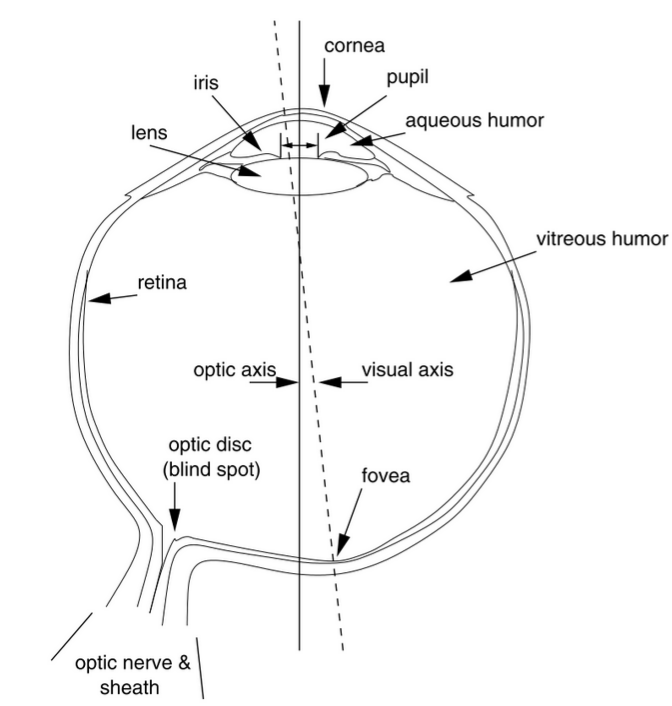
\includegraphics[width=0.7\textwidth]{eye_structure}
  \caption{Human Eye structure overview.}
  \label{fig:eye_str}
\end{figure}

In the following sub-sections, we will be discussing about Cornea, Pupil, Iris and Sclera.

\begin{homeworkSection}{(a) Cornea} % Section within problem
''The cornea is the transparent front part of the eye that covers the iris, pupil, and anterior chamber.''\footnote{Wikipedia: \url{http://en.wikipedia.org/wiki/Cornea}} Cornea acts like the outer crystal surface of a watch, protecting the inner components of the eye. Cornea itself is also made out of 5 layers listed below.

\begin{enumerate} \itemsep1pt \parskip0pt \parsep0pt
\item Corneal epithelium
\item Bowman's layer
\item Corneal stroma
\item Descemet's membrane
\item Corneal endothelium
\end{enumerate}

\end{homeworkSection}

\begin{homeworkSection}{(b) Pupil} % Section within problem
The apparently black circular opening in the center of the iris of the eye, through which light passes to the retina. It appears black because light rays entering the pupil are either absorbed by the tissues inside the eye directly, or absorbed after diffuse reflections within the eye that mostly miss exiting the narrow pupil.
\end{homeworkSection}

\begin{homeworkSection}{(c) Iris} % Section within problem
''The iris is a thin, circular structure in the eye, responsible for controlling the diameter and size of the pupil and thus the amount of light reaching the retina.'' \footnote{Wikipedia: \url{http://en.wikipedia.org/wiki/Iris_(anatomy)}} The color of the iris gives the eye its color. In optical terms, the pupil is the eye's aperture and the iris is the diaphragm that serves as the aperture stop.
\end{homeworkSection}

\begin{homeworkSection}{(d) Sclera} % Section within problem
''The sclera , also known as the white of the eye, is the opaque, fibrous, protective, outer layer of the eye containing collagen and elastic fiber.'' \footnote{Wikipedia: \url{http://en.wikipedia.org/wiki/Sclera}} In humans the whole sclera is white, contrasting with the coloured iris. The human eye is relatively rare for having an iris that is small enough for its position to be plainly visible against the sclera. This makes it easier for one individual to infer where another individual is looking, and the cooperative eye hypothesis suggests this has evolved as a method of nonverbal communication. Also, this fact is usually used in eye tracking systems.
\end{homeworkSection}

\end{homeworkProblem}

%----------------------------------------------------------------------------------------
%	Eye Trackers
%----------------------------------------------------------------------------------------

% To have just one problem per page, simply put a \clearpage after each problem

\begin{homeworkProblem}[\Roman{homeworkProblemCounter}. Eye Trackers]
Now, we come up to this question, what is an eye tracker? Any measurement device used for measuring eye position and movements is commonly known as an Eye Tracker. Eye trackers are used in research on the visual system, in psychology, in cognitive linguistics, marketing, as an input device for human computer interaction, and in product design. There are generally two types of Eye Trackers:

\begin{itemize} \itemsep1pt \parskip0pt \parsep0pt
\item Those that measure the position of the eye relative to the head
\item Those that measure the orientation of the eye in space
\end{itemize}

The second type of the trackers are typically used when we want to identify elements in a visual scene. The first usage of eye trackers recorded in human history was done in 1879 in Paris by Louis Émile Javal. He observed that reading does not involve a smooth sweeping of the eyes along the text, as previously assumed, but a series of short stops (called fixations) and quick saccades. This observation raised important questions about reading, which were explored during the 1900s: On which words do the eyes stop? For how long? When does it regress back to already seen words? \textbf{Figure \ref{fig:f_eye_t}} shows the process of reading a text which was resulted from the above mentioned experiment.

\begin{figure}[h!]
  \centering
	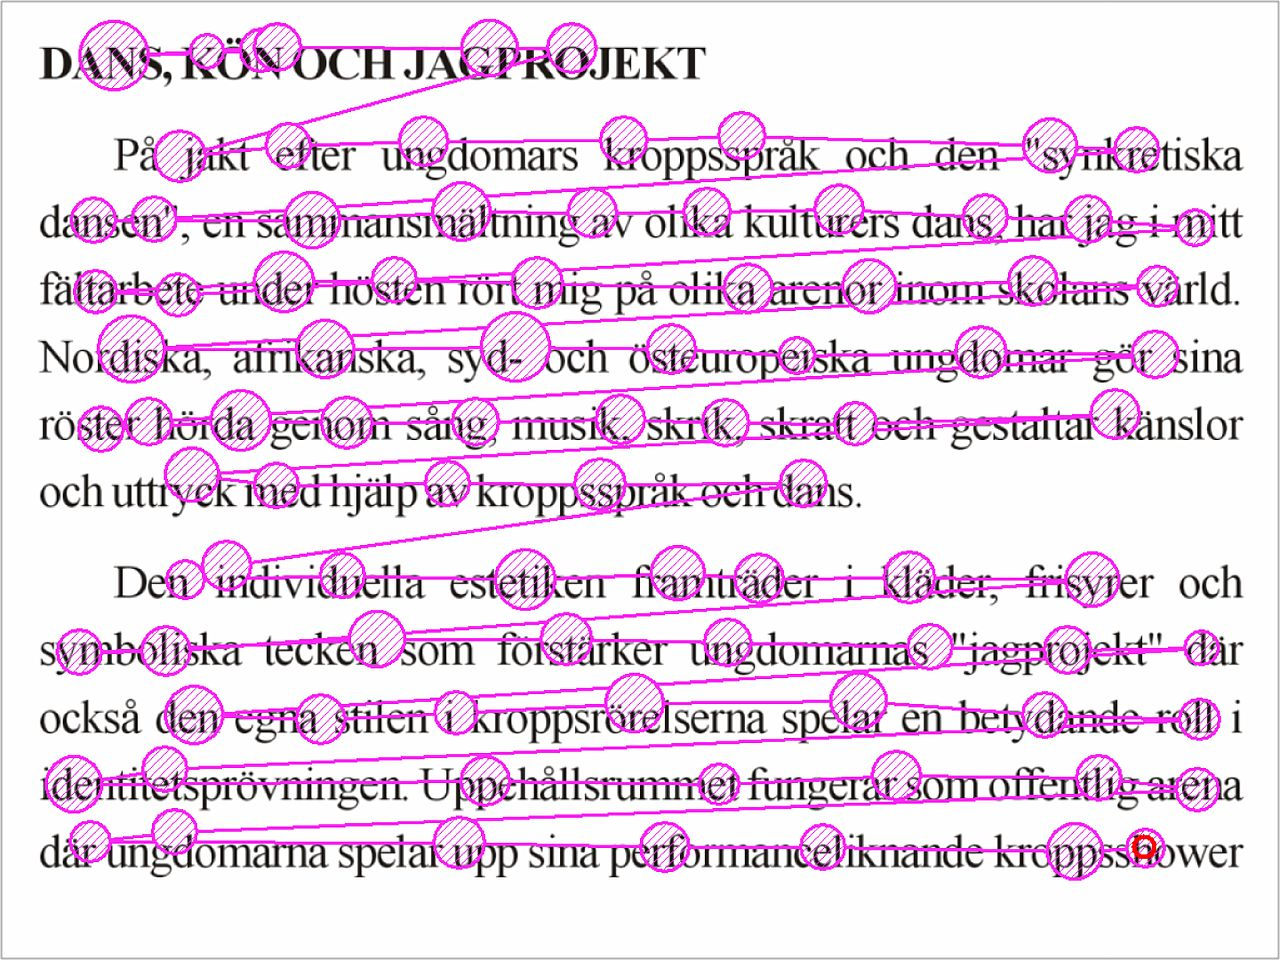
\includegraphics[width=0.7\textwidth]{first_eye_tracking}
  \caption{The result from Louis Émile Javal's research on reading a text.}
  \label{fig:f_eye_t}
\end{figure}

Another example of classic eye tracking is done in the 1950s by Alfred L. Yarbus which is considered a very important eye tracking research. He showed the task given to a subject has a very large influence on the subject's eye movement. He asked the subjects to determine some aspects of the persons entering a room like, Are the people in the image related? What are they wearing?

He also wrote about the relation between fixations and interest:
''All the records ... show conclusively that the character of the eye movement is either completely independent of or only very slightly dependent on the material of the picture and how it was made, provided that it is flat or nearly flat.'' The cyclical pattern in the examination of pictures ''is dependent not only on what is shown on the picture, but also on the problem facing the observer and the information that he hopes to gain from the picture.'' \footnote{Yarbus 1967, p. 194} \textbf{Figure \ref{fig:yarbus}} shows the results from Yarbus's experiments.

\begin{figure}[h!]
  \centering
	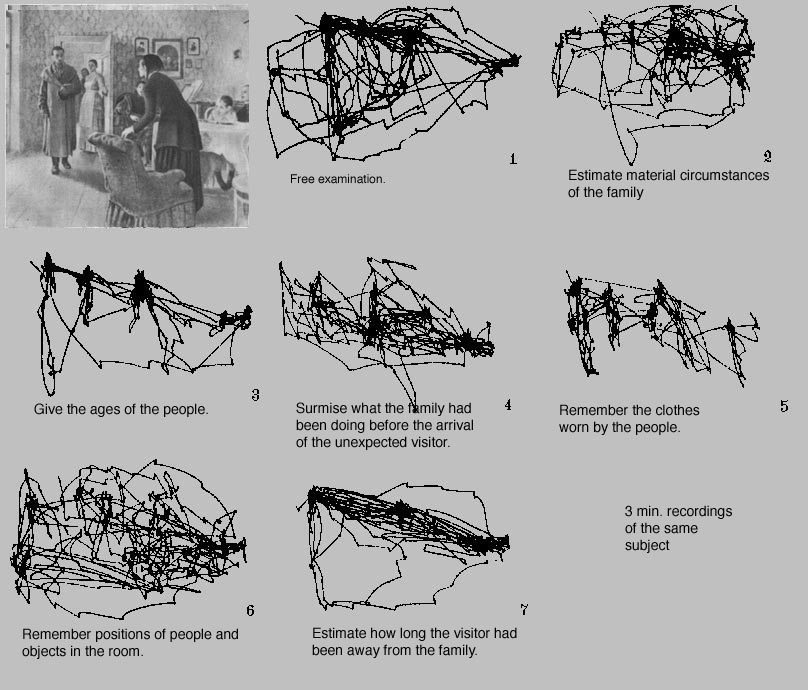
\includegraphics[width=0.7\textwidth]{yarbus}
  \caption{The result from Yarbus's experiments.}
  \label{fig:yarbus}
\end{figure}

To mention other recent usages of eye trackers, we can think of the Microsoft's HoloLens and using eye trackers in many other daily aspects of human like controlling an interface, placing advertisements in the right place and many other examples.

Now let's see a taxonomy of eye trackers.

\begin{homeworkSection}{(a) Electro-oculography (EOG)} % Section within problem
It relies on measurement of the skin’s electric potential differences, of electrodes placed around the ocular cavity. During the mid-1970s, this technique was the most widely applied eye movement method.It measures eye movements relative to head position. An example of this class is shown in \textbf{Figure \ref{fig:EOG}}.
\begin{figure}[h!]
  \centering
	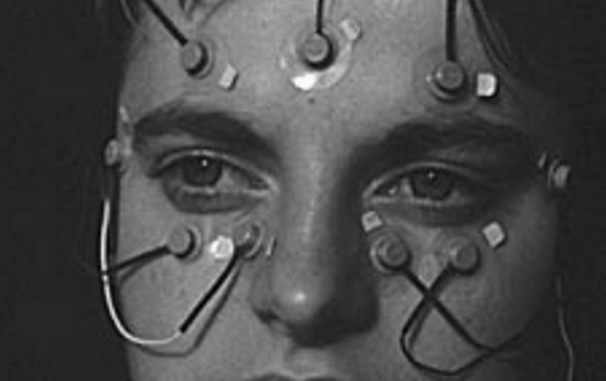
\includegraphics[width=0.5\textwidth]{EOG}
  \caption{Electro-oculography (EOG)}
  \label{fig:EOG}
\end{figure}
\end{homeworkSection}

\begin{homeworkSection}{(b) Scleral Contact Lens/Search Coil} % Section within problem
One of the most precise eye movement measurement methods which involves attaching a mechanical or optical reference object mounted on a contact lens which is then worn directly on the eye. As the problems for this method, it is considered the most intrusive method. An example of this class is shown in \textbf{Figure \ref{fig:SCL}}.
\begin{figure}[h!]
  \centering
	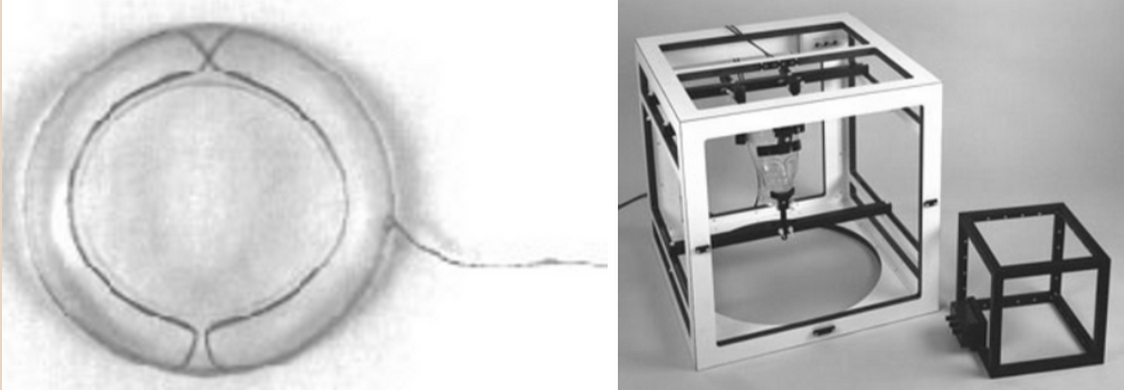
\includegraphics[width=0.7\textwidth]{SCL}
  \caption{Scleral Contact Lens/Search Coil}
  \label{fig:SCL}
\end{figure}
\end{homeworkSection}

\begin{homeworkSection}{(c) Photo-OculoGraphy (POG) or Video-OculoGraphy (VOG)} % Section within problem
These are two groups of eye trackers involving the measurement of distinguishable features of the eyes under rotation / translation. Examples of these features are,
\begin{itemize} \itemsep1pt \parskip0pt \parsep0pt
\item The apparent shape of the pupil
\item The position of the limbus (the iris-sclera boundary)
\end{itemize}
These techniques are grouped together because they often do not provide point of regard measurement.

\end{homeworkSection}

\begin{homeworkSection}{(d) Video-Based Combined Pupil/Corneal Reflection} % Section within problem

To measure the Point of Regard either,
\begin{itemize} \itemsep1pt \parskip0pt \parsep0pt
\item Subject’s head should be fixed, or
\item Multiple ocular features must be measured in order to disambiguate head movement from eye rotation
\end{itemize}

Two features that can help find the point of regard are,
\begin{itemize} \itemsep1pt \parskip0pt \parsep0pt
\item The Corneal Reflection
\item The Pupil Center
\end{itemize}
Most of the Video-based trackers utilize relatively inexpensive cameras and image processing hardware to compute the point of regard in real-time. This technique is most suitable to be used in interactive applications.
\end{homeworkSection}

We mentioned The Corneal Reflections or also called The Purkinje Images. Purkinje Images are reflections of objects from the structure of the eye. At least four Purkinje images are usually visible:
\begin{enumerate} \itemsep1pt \parskip0pt \parsep0pt
\item The first Purkinje image (P1) is the reflection from the outer surface of the cornea
\item The second Purkinje image (P2) is the reflection from the inner surface of the cornea
\item The third Purkinje image (P3) is the reflection from the outer (anterior) surface of the lens
\item The fourth Purkinje image (P4) is the reflection from the inner (posterior) surface of the lens
\end{enumerate}

We need two points of reference on the eye to separate eye movements from head movements. As the positional difference between the pupil center and corneal reflection \textbf{changes with pure eye rotation} but \textbf{remains relatively constant with minor head movements} most Video-Based eye trackers measure the First and sometimes the Fourth (in generation-V systems) Corneal Reflections and based on these measurements, they separate translational and rotational eye movements. \textbf{Figure \ref{fig:PUR}} shows the first, third and the fourth Purkinje Images.

\begin{figure}[h!]
  \centering
	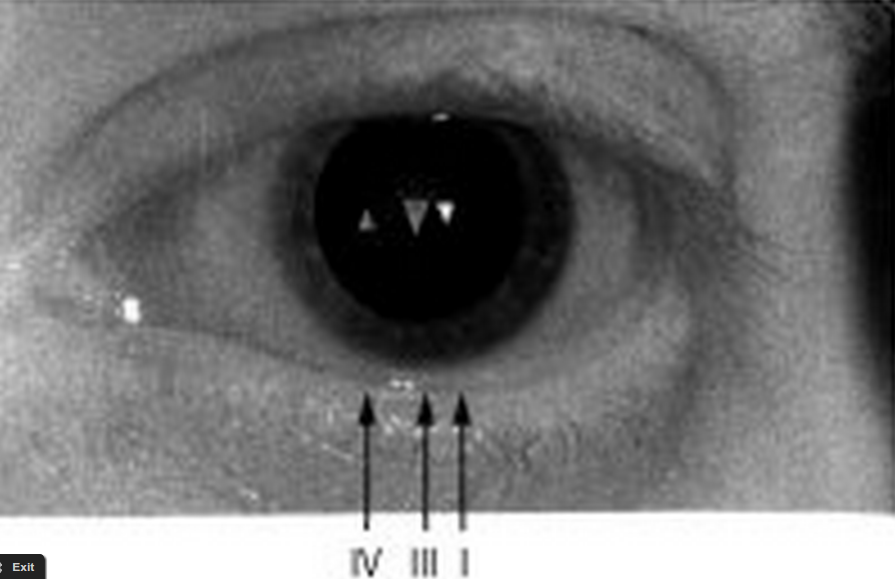
\includegraphics[width=0.4\textwidth]{pur}
  \caption{the first, third and the fourth Purkinje Images}
  \label{fig:PUR}
\end{figure}

\end{homeworkProblem}

%----------------------------------------------------------------------------------------
%	Starburst
%----------------------------------------------------------------------------------------

% To have just one problem per page, simply put a \clearpage after each problem

\begin{homeworkProblem}[\Roman{homeworkProblemCounter}. Starburst]

The primary obstacle of integrating eye movements into today’s interfaces is the availability of a reliable, low-cost open-source eye-tracking system. Towards making such a system available to interface designers, a hybrid eye tracking algorithm that integrates feature-based and model-based approaches  has been introduced in this study is made available in an open-source package. This algorithm is referred to as “starburst” because of the novel way in which pupil features are detected. This starburst algorithm is more accurate than pure feature-based approaches yet is significantly less time consuming than pure model-based approaches.

The bird eye view of the algorithm is as depicted in \textbf{Figure \ref{fig:BIRD}}. In the following subsections, the different parts of this algorithm are explained in more detail.

\begin{figure}[h!]
  \centering
	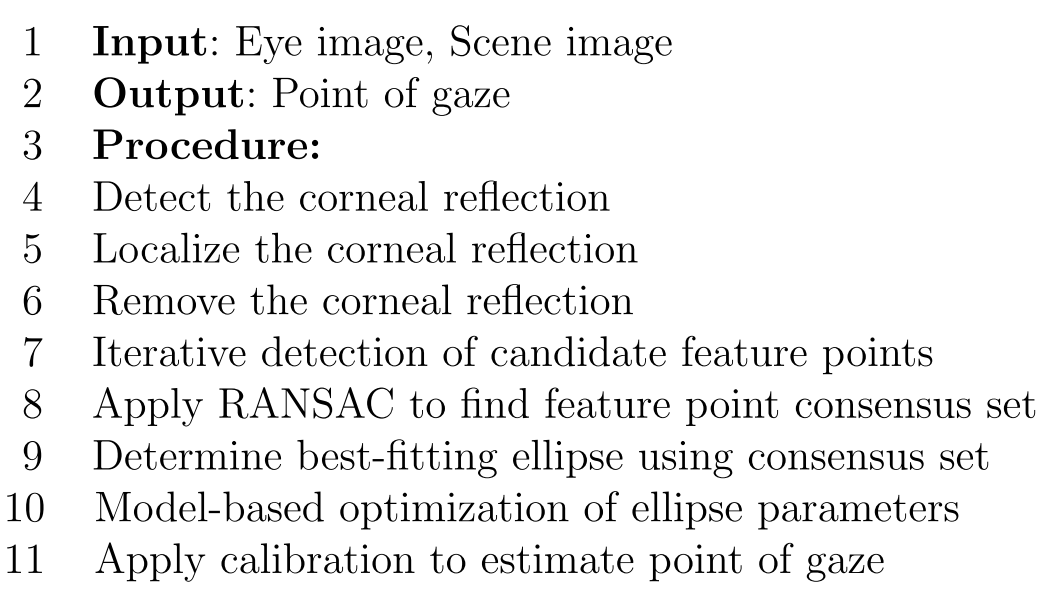
\includegraphics[width=0.7\textwidth]{bird}
  \caption{Starburst Algorithm}
  \label{fig:BIRD}
\end{figure}


\begin{homeworkSection}{(a) Noise Reduction}
Due to the use of cheap consumer grade CCD cameras, we need to start by reducing the noise in the images. There Are two types of noise in the images:

\begin{itemize} \itemsep1pt \parskip0pt \parsep0pt
\item Shot noise: Reduced by using a 5x5 Gaussian filter with a standard deviation of 2 pixels.
\item Line noise: This noise is reduced by applying a normalization factor (C) line by line to shift the mean intensity of the line to the running average derived from the previous frame. 
\end{itemize}
An example of the effect which the noise reduction process has on the image can be seen in \textbf{Figure \ref{fig:NOISE}}.

\begin{figure}[h!]
  \centering
	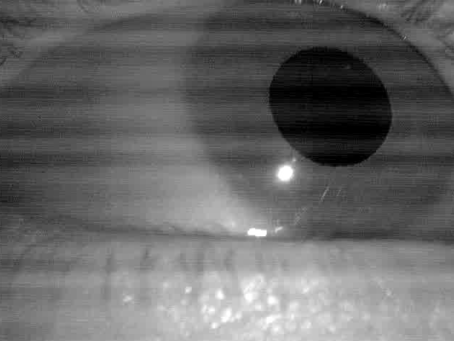
\includegraphics[width=0.3\textwidth]{noise1}
	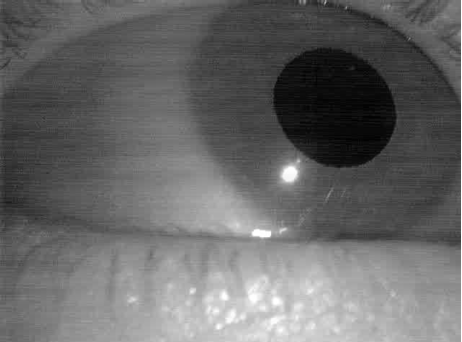
\includegraphics[width=0.3\textwidth]{noise2}
  \caption{Noise Reduction effect}
  \label{fig:NOISE}
\end{figure}
\end{homeworkSection}

%%%%%%%%%%%%%%%%%%%%%%%%%%%%%%%%%%%%%%%%%%%%%%%%%%
\begin{homeworkSection}{(b) Corneal reflection detection and localization}

\end{homeworkSection}
%-------------------------------------------------

%%%%%%%%%%%%%%%%%%%%%%%%%%%%%%%%%%%%%%%%%%%%%%%%%%
\begin{homeworkSection}{(c) Corneal reflection removal}

\end{homeworkSection}
%-------------------------------------------------

%%%%%%%%%%%%%%%%%%%%%%%%%%%%%%%%%%%%%%%%%%%%%%%%%%
\begin{homeworkSection}{(d) Pupil contour detection}

\end{homeworkSection}
%-------------------------------------------------

%%%%%%%%%%%%%%%%%%%%%%%%%%%%%%%%%%%%%%%%%%%%%%%%%%
\begin{homeworkSection}{(e) Ellipse fitting}

\end{homeworkSection}
%-------------------------------------------------

%%%%%%%%%%%%%%%%%%%%%%%%%%%%%%%%%%%%%%%%%%%%%%%%%%
\begin{homeworkSection}{(f) Model-based optimization}

\end{homeworkSection}
%-------------------------------------------------

%%%%%%%%%%%%%%%%%%%%%%%%%%%%%%%%%%%%%%%%%%%%%%%%%%
\begin{homeworkSection}{(g) Calibration}

\end{homeworkSection}
%-------------------------------------------------

\end{homeworkProblem}

\end{document}
